\section{Using the platform}

In order to use the platform a developer have to perform two steps.
\begin{itemize}
\item Add the host language support. To do this it is necessary to provide the module which for a source code on the host language can build a generalized CFG and mark target nodes in it. Generalized control flow graph specification is defined by the platform. The result of this module's work will be passed to the Approximation component as an input.
\item Add the support of the string-embedded language through the implementation of the common interface. To achieve this it is necessary to provide the lexical specification (needed for lexer generation) and the grammar (needed for parser generation) of the embedded language. After the lexer and parser are created developer can use the standard implementation of the interface functions.
\end{itemize}

After these steps are performed a developer obtains the tool which supports the desired string-embedded language inside the desired host one. An embedded code syntax highlighting, matching parentheses highlighting, and static errors detection becomes available for these pair of languages. Microsoft Visual Studio with the ReSharper\footnote{ReSharper is plugin to Microsoft Visual Studio, extending standard IDE functionality. Site: \url{http://www.jetbrains.com/resharper/}} plugin is used as a target IDE. The functionality currently available is not very rich, but the platform's architecture is designed for further extension.

Currently available functions can be configured by the user. Syntax highlighting can be configured by specifying the mapping between each token type and the color it should be highlighted with. Also user can choose which tokens are considered as paired: for each pair "left" and "right" elements are to be set (opening and closing parentheses, for instance). If a caret in the editor is located near one of the paired elements the other element corresponding to it will be highlighted.

\subsection{Evaluation}

To test the platform the tools for embedding T-SQL and arithmetic expressions language (called Calc) in C\# and JavaScript were implemented. The tools are designed to work on Microsoft .NET platform. The most popular IDE for the .NET platform is Microsoft Visual Studio. By default it has no string-embedded languages support. The implemented tools were integrated as extensions to ReSharper~--  a plugin to Microsoft Visual Studio, which extends the the default functionality of the IDE.

ReSharper has a freely available SDK containing most of the ReSharper's functionality, in particular the capability to build control flow graphs for the source code. The modules for building C\# and JavaScript specific CFGs and converting them to generalized ones were implemented using the SDK.

For strings with embedded code searching, an algorithm based on the special predefined set of functions (or methods) usage was implemented. These functions are called hotspots. What is special about these functions is that we know they expect a string with embedded code as an argument. In the source code we search calls of these hotspot functions and the arguments of the calls are set to be target expressions. The main idea of the approach is based on the fact, that the programs that construct the strings with embedded code often use some subsystem to execute it. The method \verb|"execute"| of the \verb|java.SQL.Statement| interface that is used in Java programs to execute SQL queries via JDBC technology can be considered as an example. In general the described approach does not always work correctly, but relative implementation simplicity is it's undoubted advantage.

The information about hotspots is stored in the configuration .xml file. For each hotspot it contains corresponding function's signature and the name of the embedded language the hotspot corresponds to. In the case of T-SQL a hotspot is a method or function named \verb|ExecuteImmediate|, in case of Calc -- named \verb|Eval|. It should be noted that hotspots for different embedded languages can occur in the same analyzed file with the source code.

Lexical and parser specifications were built for Calc and a subset of T-SQL languages. The lexer and parser were generated using these specifications. Xml files for syntax highlighting and set of classes for ReSharper integration were created during the parser generation.

\textbf{Syntax highlighting.} The example of T-SQL and Calc languages support in C\# is shown in Figure~\ref{highlighting}. Each language is highlighted separately: numbers in T-SQL query and in Calc expressions have different colors. Note the value of the \verb|"expr"| variable is formed in a loop using conditional statement and \textit{TrueCaseStr} function invocation. Plugin handles all these host language constructions for strings building so highlighting is performed even inside \textit{TrueCaseStr} method. 

\begin{figure}[h!]
    \begin{center}
        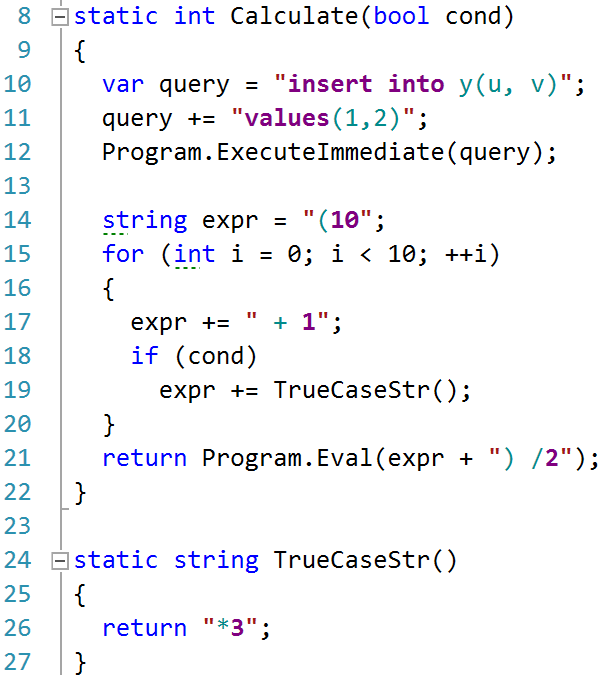
\includegraphics[scale=0.4]{Figures/sql_and_calc_cycle.PNG}
    \end{center}
    \caption{T-SQL and Calc syntax highlighting}
    \label{highlighting}
\end{figure}

\textbf{Static errors detection.} Plugin can find lexical errors and errors related to language semantics. In figure~\ref{static_error} \verb|"varY"| variable (line 22) is underlined as undefined because there exists the path that does not contain \verb|"varY"| declaration (if \verb|cond| parameter value is false).

\begin{figure}[h!]
    \begin{center}
        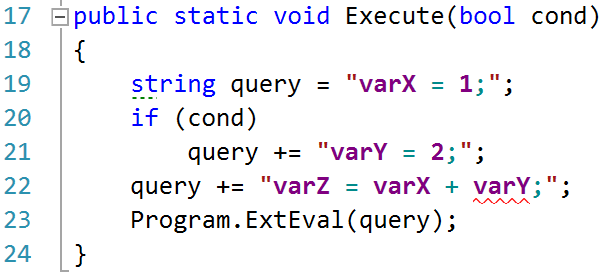
\includegraphics[scale=0.4]{Figures/Undefined_variable.PNG}
    \end{center}
    \caption{Static errors detection}
    \label{static_error}
\end{figure}

\textbf{Matching parenthesis highlighting.} Matching parenthesis highlighting improves the code readability. If a caret in the text editor is located near the one of paired symbols then the plugin should highlight it and it's matching symbol. The situation with dynamically generated expressions is different because one symbol in a pair may have several matching ones. Such a case is shown in Figure~\ref{brace1}. Opening brace (line 27) has two matching closing braces (lines 30 and 32) so three elements are highlighted. At the same time each closing brace has only one matching opening brace (Figure~\ref{brace2}).

\begin{figure}[h!]
  \begin{center}
    \begin{subfigure}[t]{0.2\textwidth}    
        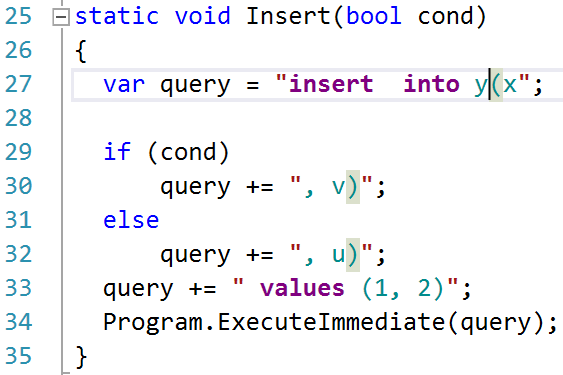
\includegraphics[scale=0.3]{Figures/brackets_one_to_many.PNG}    
    \caption{Multiple matches}
    \label{brace1}
    \end{subfigure}
	~\qquad
    \begin{subfigure}[t]{0.2\textwidth}      
            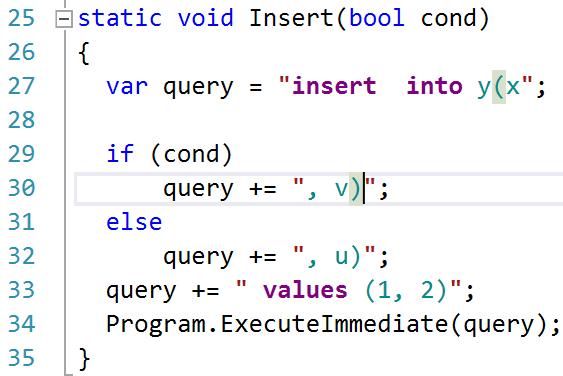
\includegraphics[scale=0.3]{Figures/brackets_one_to_one.PNG}        
        \caption{Single match}
        \label{brace2}
    \end{subfigure}
    \caption{Parenthesis highlighting}
    \label{braces}
  \end{center}
\end{figure}